\subsubsection{UC1 - Addestramento del sistema}%
\label{sssec:uc1}

\begin{figure}[h!]
  \begin{center}
    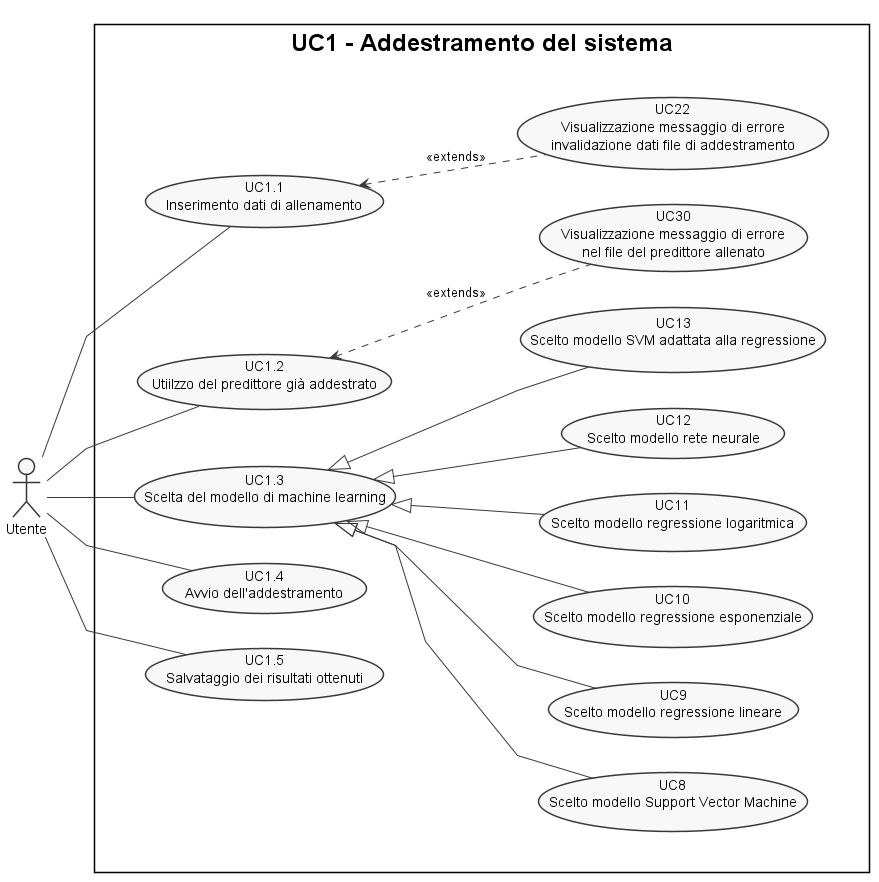
\includegraphics[width=15cm]{uc1.png}\\
    \caption{UC1 - Addestramento del sistema}%
    \label{fig:uc1}
  \end{center}
  \end{figure}

\begin{itemize}
  \item \textbf{Attore primario}: Utente;
  \item \textbf{Descrizione}: Per creare il file JSON contenente il predittore da dare al sistema di monitoraggio Grafana l'utente deve creare un file contenente i dati, scegliere il modello di machine learning da utilizzare e infine deve avviare l'addestramento;
  \item \textbf{Precondizione}: L'utente deve avere dei dati e sapere che modello utilizzare;
  \item \textbf{Scenario principale}:
  \begin{enumerate}
    \item L'utente inserisce i dati (UC1.1);
    \item L'utente utilizza un predittore già addestrato, se ne è in possesso (UC1.2);
    \item L'utente sceglie il modello di machine learning (UC1.3);
    \item L'utente avvia l'addestramento (UC1.4);
    \item L'utente crea un file contenente il predittore (UC1.5).
  \end{enumerate}
    \item \textbf{Postcondizione}: Si è ottenuto un file contente il predittore da dare a Grafana.
\end{itemize}

\paragraph{UC1.1 - Inserimento dati di allenamento}
\label{para:uc1.1}
\begin{itemize}
  \item \textbf{Attore primario}: Utente;
  \item \textbf{Descrizione}: L'utente inserisce i dati raccolti da un database in un file CSV;
  \item \textbf{Precondizione}: L'utente è in possesso di dati;
  \item \textbf{Scenario principale}:
  \begin{enumerate}
    \item L'utente carica i dati all'interno del file CSV;
    \item I dati vengono caricati nel sistema.
  \end{enumerate}
  \item \textbf{Postcondizione}: Il file CSV contiene i dati raccolti dall'utente;
  \item \textbf{Estensioni}: UC1.1 viene esteso nel caso d'uso UC22 con la visualizzazione del messaggio di errore quando viene fornito un file di addestramento non valido.
\end{itemize}

\paragraph{UC1.2 - Utilizzo del predittore già addestrato}
\label{para:uc1.2}
\begin{itemize}
  \item \textbf{Attore primario}: Utente;
  \item \textbf{Descrizione}: L'utente utilizza il file JSON contenente il predittore addestrato in un'applicazione esterna;
  \item \textbf{Precondizione}: L'utente ha a disposizione il predittore già allenato;
  \item \textbf{Scenario principale}: L'utente, qualora possieda un predittore precedentemente allenato, lo carica nel sistema;
  \item \textbf{Postcondizione}: L'utente ha a disposizione un predittore già addestrato;
  \item \textbf{Estensioni}: UC1.2 viene esteso nel caso d'uso UC30 con la visualizzazione del messaggio di errore quando si tenta di caricare un predittore in un formato non valido.
\end{itemize}

\paragraph{UC1.3 - Scelta del modello di machine learning}%
\label{para:uc1.3}
\begin{itemize}
  \item \textbf{Attore primario}: Utente;
  \item \textbf{Descrizione}: L'utente decide che tipo di machine learning utilizzare tra SVM, RL, regressione esponenziale, regressione logaritmica, SVM adattata alla regressione e rete neurale;
  \item \textbf{Precondizione}:
  \begin{enumerate}
    \item L'inserimento dei dati è avvenuto correttamente (UC1);
    \item L'utente ha a disposizione i tre modelli di machine learning.
  \end{enumerate}
  \item \textbf{Scenario principale}: L'utente, avente un file contenente i dati, decide che modello di machine learning utilizzare tra SVM, RL, regressione esponenziale, regressione logaritmica, SVM adattata alla regressione o rete neurale;
  \item \textbf{Postcondizione}: L'utente ha scelto un modello di machine learning;
  \item \textbf{Generalizzazioni}: UC1.3 viene generalizzato dai casi d'uso  UC8, UC9, UC10, UC11, UC12 e UC13.
\end{itemize}

\paragraph{UC1.4 - Avvio dell'addestramento}
\label{para:uc1.4}
\begin{itemize}
  \item \textbf{Attore primario}: Utente;
  \item \textbf{Descrizione}: L'utente utilizzando la libreria e i dati ottiene il predittore;
  \item \textbf{Precondizione}:
  \begin{enumerate}
    \item L'utente ha a disposizione il file contenente i dati (UC1);
    \item L'utente ha scelto un modello di machine learning.
  \end{enumerate}
  \item \textbf{Scenario principale}: Avendo a disposizione il file con i dati e avendo scelto un modello avviene l'addestramento;
  \item \textbf{Postcondizione}: Si è ottenuto il predittore.
\end{itemize}

\paragraph{UC1.5 - Salvataggio del risultati ottenuti}
\label{para:uc1.5}
\begin{itemize}
  \item \textbf{Attore primario}: Utente;
  \item \textbf{Descrizione}: I risultati ottenuti vengono salvati nel file JSON, riportando anche la tipologia di modello di machine learning utilizzato;
  \item \textbf{Precondizione}:
  \begin{enumerate}
    \item L'utente ha inserito i dati(UC1.1);
    \item L'utente ha deciso che modello di machine learning  utilizzare(UC1.3).
  \end{enumerate}
  \item \textbf{Scenario principale}: Una volta ottenuti i risultati dall'addestramento, l'utente salva i dati e il modello utilizzato nel file JSON;
  \item \textbf{Postcondizione}: Il file contiene sia il predittore che il modello utilizzato.
\end{itemize}

